\chapter{Постановка задачи}
Население подразделяется на различные группы в соответствии с их экономическими или индивидуальными характеристиками. Это население можно классифицировать по цвету кожи на белых и черных, по уровню дохода на богатых и бедных , по образованию на образованных и не образованных и.т.д. В ряде стран таких как США или страны Европы, сосуществование групп населения, принадлежащих различным расам, порождало и порождает серьезные социальные проблемы и поэтому изучалось с различных точек зрения.

Взаимодействие подобных групп населения, внутри единой городской агломерации, может быть описано на качественном уровне, с помощью системы из нескольких, нестационарных нелинейных дифференциальных уравнений диффузионного типа. Для простоты рассмотрено только две группы, обозначаемые как группа 1 и группа 2:
\begin{empheq}[left=\empheqlbrace]{equation}
    \label{eq1:system}
    \begin{aligned}
        \frac{\p u}{\p t} = L_{1} u + F_{1} (u,v) \\
        \frac{\p v}{\p t} = L_{2} v + F_{2} (u,v)
    \end{aligned}
\end{empheq}
где искомые функции $u=u(x_{1},x_{2},t)$ и $v=v(x_{1},x_{2},t)$ по смыслу определяют соответственно плотности 1-ой и 2-ой групп населения в точке $(x_{1},x_{2})$ в момент времени $t$.

Функция <<взаимодействия>> $F_{s}(u,v) : (s=1,2) $ (источника), в этой системе уравнений играет ключевую роль, так как она и влияет на всю модель непосредственно. Подробности коэффициентов которых будут изложены в последней главе (\ref{ch3:results}). 

В системе (\ref{eq1:system}) дифференциальный оператор (диффузионный член) $L_{s}: (s = 1,2)$ присутствующий в правых частях, отображает эффект географической диффузии населения и имеет следующий вид:
\begin{equation*}
    L_{s} = div(K_{s} \ grad ),\quad s = 1,2
\end{equation*}
дивергентный вид которого описывается как: 
\begin{equation*}
    div(K_{s} \ grad ) = \nabla \left(K_{s} \cdot \nabla \right) =  \frac{\p }{\p x_{1}} \left(K_{s} \frac{\p .}{\p x_{1}} \right) + \frac{\p }{\p x_{2}} \left(K_{s} \frac{\p .}{\p x_{2}} \right), \quad  s = 1,2
\end{equation*}

 Предполагается, что коэффициенты $K_{1} = K_{1}(u,v),\ K_{2} = K_{2}(u,v)$ , т.е. зависят от неизвестных функций, что автоматически означает нелинейность системы уравнений.\\ Зависимость этих коэффициентов от неизвестных функций и определяет нелинейность рассматриваемой задачи и все трудности ее решения, которые с этим связаны.

Система (\ref{eq1:system}) решается в области $\Omega$ (рис. \ref{fig:omega}).
% \begin{equation*}
%     \Omega = \{ (0<x_{1}<l_{1})\times (0<x_{2}<l_{2})\times (0<t<T_{\max } )\} .
% \end{equation*}

\begin{figure}[ht!]
    \centering
    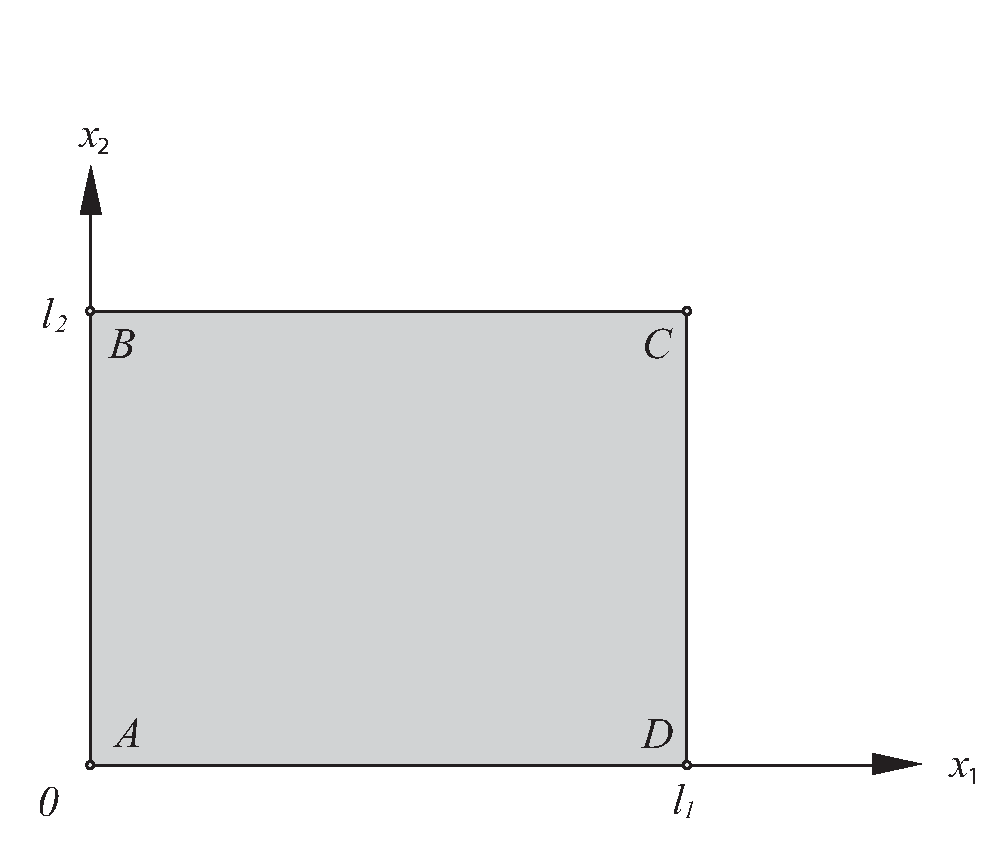
\includegraphics[scale = 0.5]{oblast}
    \captionsetup{justification=centering,margin=2cm}
    \caption{Область решения задачи: $x_{1},x_{2}$ - декартовы координаты;\\ $l_{1}$ - ширина области по $x_{1}$ , $l_{2}$ - ширина области по $x_{2}$;\\ A,B,C,D - граничные точки}
    \label{fig:omega}
\end{figure}

Для завершения математической постановки задачи для дифференциальной системы (\ref{eq1:system}) необходимо также задать начальные и граничные условия.

\section{Начальные условия}
\begin{empheq}[left=\empheqlbrace]{equation}
    \label{eq1:init}
    \begin{aligned}
        u(x_{1},x_{2},t)\vert_{t=0} &=u_{0} (x_{1},x_{2})\\
        v(x_{1},x_{2},t)\vert_{t=0} &=v_{0} (x_{1},x_{2})
    \end{aligned}
    \qquad \qquad
\end{empheq}
таким образом начальная городская структура описывается функциями $u_{0}(x_{1},x_{2})$ и $v_{0}(x_{1},x_{2})$.


\section{Граничные условия}  
\paragraph{Условия первого рода:}
\begin{empheq}[left=\empheqlbrace]{equation}
    \label{eq1:cond1}
    \begin{aligned}
		\left. u(x_{1},x_{2},t)\right|_{\Gamma} &= \varphi_1 \\
		\left. v(x_{1},x_{2},t)\right|_{\Gamma} &= \varphi_2 
    \end{aligned}
    \qquad (x_{1},x_{2}) \in \; \Gamma
\end{empheq}
задается распределение плотности населения на границах области для каждого момента времени. Здесь $\varphi_{s}: (s = 1,2)$ так же может зависеть времени $\varphi_{s} = \varphi_{s}(t)$. 

\paragraph{Условия второго рода:}

\begin{empheq}[left=\empheqlbrace]{equation}
    \label{eq1:cond2}
    \begin{aligned}
		K_{1}\left. \frac{\partial u}{\partial n} \; \right|_{\Gamma } \quad &=\varphi_1\\
		K_{2}\left. \frac{\partial v}{\partial n} \; \right|_{\Gamma } \quad &=\varphi_2
    \end{aligned}
    \qquad (x_{1},x_{2}) \in \; \Gamma
\end{empheq}
то есть мы допускаем <<поток>> населения через границу городского пространства, или же ограничиваем его поставив производную равную нулем.
\paragraph{Условия третьего рода:}

\begin{empheq}[left=\empheqlbrace]{equation}
    \label{eq1:cond3}
    \begin{aligned}
    	\left.\left(A_{1} u + K_{1} \frac{\partial u}{\partial n} \right) \right|_{\Gamma } &=\varphi_1\\
    	\left.\left(A_{2} v + K_{2} \frac{\partial v}{\partial n} \right) \right|_{\Gamma } &=\varphi_2\\ 	
    \end{aligned}
    \quad (x_{1},x_{2}) \in \Gamma \quad A_{s} = const, \; s = 1,2,
\end{empheq}
как и в физических задачах тепло-массы переноса, обмен с внешней средой имеет место быть. Трактовать это можно тем что не возможно ограничить поток население в одну сторону, таким образом такие условия, придают модели немало важную составляющую.

В краевых условиях второго и третьего рода (\ref{eq1:cond2}) - (\ref{eq1:cond3}), производная $ \frac{\p .}{\p n} $ обозначает нормальную производную от искомой функции по вектору внешней единичной нормали к соответствующему участку границы $ \Gamma = \{AB \cup BC \cup CD \cup AD \} $, т.е.:

\begin{itemize}
\item на участке границы $AB$ это: \; $ \left. \frac{\p .}{\p n} \right|_{\Gamma} = - \left. \frac{\p .}{\p x_{1}} \right|_{AB}
\; (x_{1},x_{2}) \in AB : \{ x_{1} = 0,\; 0 < x_{2} < l_{2} \}$
\item на участке границы $BC$ это: \; $ \left. \frac{\p .}{\p n} \right|_{\Gamma} = \phantom{-} \left. \frac{\p .}{\p x_{2}} \right|_{BC}
\; (x_{1},x_{2}) \in BC : \{ 0 < x_{1} < l_{1},\; x_{2} = l_{2} \}$
\item на участке границы $CD$ это: \; $ \left. \frac{\p .}{\p n} \right|_{\Gamma} = \phantom{-} \left. \frac{\p .}{\p x_{1}} \right|_{CD}
\; (x_{1},x_{2}) \in CD : \{ x_{1} = l_{1},\; 0 < x_{2} < l_{2} \}$
\item на участке границы $AD$ это: \; $ \left. \frac{\p .}{\p n} \right|_{\Gamma} = -\left. \frac{\p .}{\p x_{2}} \right|_{AD}
\; (x_{1},x_{2}) \in AD : \{ 0 < x_{1} < l_{1},\; x_{2} = 0 \}$
\end{itemize}

В итоге имеем систему из дифференциальных уравнений (\ref{eq1:system}) с начальными(\ref{eq1:init})  и граничными условиями трех видов (\ref{eq1:cond1} - \ref{eq1:cond3}). Параметры и коэффициенты которых  (параметры источника $F_{\alpha}(u,v)$, параметры граничных условий и коэффициент диффузии $K_{\alpha}(u,v)$), если задавать нужным образом, и будут влиять на решение этой системы. К чему собственно и сводится математическая модель взаимодействия групп населения, это поиск таких параметров системы, которые удовлетворяют (<<воле экспериментатора>>) искомому решению.